%%%%%%%%%%%%%%%%%%%%%%%%%%%%%%%%%%%%%%%%%
% Beamer Presentation
% LaTeX Template
% Version 1.0 (10/11/12)
%
% This template has been downloaded from:
% http://www.LaTeXTemplates.com
%
% License:
% CC BY-NC-SA 3.0 (http://creativecommons.org/licenses/by-nc-sa/3.0/)
%
%%%%%%%%%%%%%%%%%%%%%%%%%%%%%%%%%%%%%%%%%

%----------------------------------------------------------------------------------------
%	PACKAGES AND THEMES
%----------------------------------------------------------------------------------------

%\documentclass[UTF8,aspectratio=169,14pt]{ctexbeamer}
\documentclass[UTF8,aspectratio=169]{ctexbeamer}
\usepackage{hyperref}
\hypersetup{
	colorlinks=true,
	linkcolor=red,
	anchorcolor=blue,
	citecolor=green
}

\mode<presentation> {
	
	% The Beamer class comes with a number of default slide themes
	% which change the colors and layouts of slides. Below this is a list
	% of all the themes, uncomment each in turn to see what they look like.
	
	%\usetheme{default}
	%\usetheme{AnnArbor}
	%\usetheme{Antibes}
	%\usetheme{Bergen}
	%\usetheme{Berkeley}
	%\usetheme{Berlin}
	%\usetheme{Boadilla}
	%\usetheme{CambridgeUS}
	%\usetheme{Copenhagen}
	%\usetheme{Darmstadt}
	%\usetheme{Dresden}
	%\usetheme{Frankfurt}
	%\usetheme{Goettingen}
	%\usetheme{Hannover}
	%\usetheme{Ilmenau}
	%\usetheme{JuanLesPins}
	%\usetheme{Luebeck}
	\usetheme{Madrid}
	%\usetheme{Malmoe}
	%\usetheme{Marburg}
	%\usetheme{Montpellier}
	%\usetheme{PaloAlto}
	%\usetheme{Pittsburgh}
	%\usetheme{Rochester}
	%\usetheme{Singapore}
	%\usetheme{Szeged}
	%\usetheme{Warsaw}
	
	% As well as themes, the Beamer class has a number of color themes
	% for any slide theme. Uncomment each of these in turn to see how it
	% changes the colors of your current slide theme.
	
	%\usecolortheme{albatross}
	%\usecolortheme{beaver}
	%\usecolortheme{beetle}
	%\usecolortheme{crane}
	%\usecolortheme{dolphin}
	%\usecolortheme{dove}
	%\usecolortheme{fly}
	%\usecolortheme{lily}
	%\usecolortheme{orchid}
	%\usecolortheme{rose}
	%\usecolortheme{seagull}
	%\usecolortheme{seahorse}
	%\usecolortheme{whale}
	%\usecolortheme{wolverine}
	
	%\setbeamertemplate{footline} % To remove the footer line in all slides uncomment this line
	%\setbeamertemplate{footline}[page number] % To replace the footer line in all slides with a simple slide count uncomment this line
	
	%\setbeamertemplate{navigation symbols}{} % To remove the navigation symbols from the bottom of all slides uncomment this line
}

\usepackage{graphicx} % Allows including images
\graphicspath{{./figs/}}
\usepackage{booktabs} % Allows the use of \toprule, \midrule and \bottomrule in tables
\usepackage{longtable}
\usepackage{listings}
\usepackage{xcolor}
\lstset{numbers=left, %设置行号位置
	numberstyle=\tiny, %设置行号大小
	keywordstyle=\color{blue}, %设置关键字颜色
	commentstyle=\color[cmyk]{1,0,1,0}, %设置注释颜色
	frame=single, %设置边框格式
	escapeinside=``, %逃逸字符(1左面的键),用于显示中文
	%breaklines, %自动折行
	extendedchars=false, %解决代码跨页时,章节标题,页眉等汉字不显示的问题
	xleftmargin=2em,xrightmargin=2em, aboveskip=1em, %设置边距
	tabsize=4, %设置tab空格数
	showspaces=false %不显示空格
}
% Fonts
% \usepackage{libertine}
% \setmonofont{Courier}
\setCJKsansfont[ItalicFont=Noto Serif CJK SC Black, BoldFont=Noto Sans CJK SC Black]{Noto Sans CJK SC}
\setmainfont[Ligatures={Common,TeX}]{Linux  Libertine O}
\setmonofont[SmallCapsFont={Latin Modern Mono Caps}]{Latin Modern Mono Light}
\setsansfont{Linux Biolinum O}

\logo{
\includegraphics[width=0.55cm,height=0.55cm]{../../thcs-logo.png}}

%----------------------------------------------------------------------------------------
%	TITLE PAGE
%----------------------------------------------------------------------------------------

\title[第11讲]{第11讲 :Scalable Synchronization on Shared-Memory Multiprocessors} % The short title appears at the bottom of every slide, the full title is only on the title page
\subtitle{第一节:Introduction }
\author{陈渝} % Your name
\institute[清华大学] % Your institution as it will appear on the bottom of every slide, may be shorthand to save space
{
	清华大学计算机系 \\ % Your institution for the title page
	\medskip
	\textit{yuchen@tsinghua.edu.cn} % Your email address
}
\date{\today} % Date, can be changed to a custom date



\begin{document}

\begin{frame}
\titlepage % Print the title page as the first slide
\end{frame}

%\begin{frame}
%\frametitle{提纲} % Table of contents slide, comment this block out to remove it
%\tableofcontents % Throughout your presentation, if you choose to use \section{} and \subsection{} commands, these will automatically be printed on this slide as an overview of your presentation
%\end{frame}
%
%%----------------------------------------------------------------------------------------
%%	PRESENTATION SLIDES
%%----------------------------------------------------------------------------------------
%
%%------------------------------------------------
%\section{第一节:课程概述} % Sections can be created in order to organize your presentation into discrete blocks, all sections and subsections are automatically printed in the table of contents as an overview of the talk
%%------------------------------------------------
%-------------------------------------------------
\begin{frame}[plain]
	\frametitle{Introduction}
	
	
	
	\begin{columns}
		
		\begin{column}{.5\textwidth}
			\centering
			
			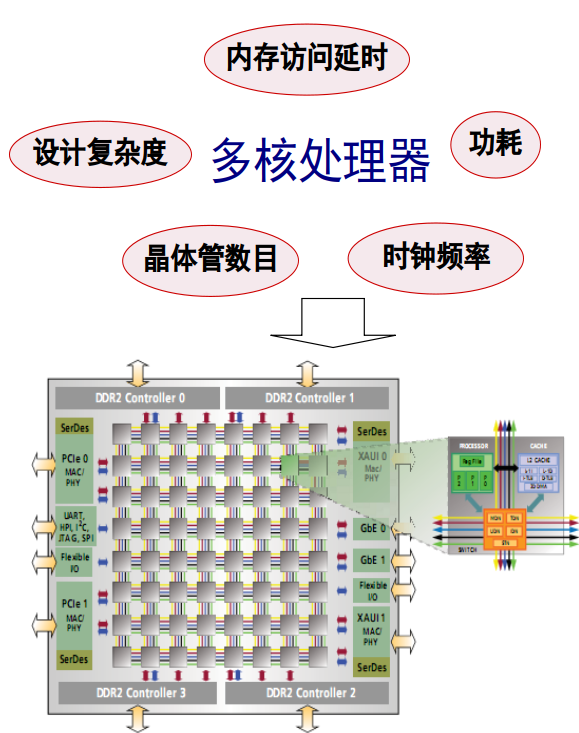
\includegraphics[width=.7\textwidth]{multicore-arch}

		\end{column}
		
		\begin{column}{.5\textwidth}
			
			\Large

			\begin{itemize}
				\item 工业界普遍采用
				\item Intel/AMD/IBM/ARM/RISC-V
				\item 服务器/PC/笔记本/嵌入式系统
			
			\end{itemize}
			
		\end{column}
		
		
	\end{columns}
	
\tiny ref:
Some info are from

Paul McKenney (IBM) Tom Hart (University of Toronto), Frans Kaashoek (MIT), 
Daniel J. Sorin "A Primer on Memory Consistency and Cache Coherence", Fabian Giesen "Cache coherency primer", Mingyu Gao(Tsinghua),Yubin Xia(SJTU)
	
\end{frame}


%----------------------------------------------
\begin{frame}[plain]	
	\frametitle{Introduction}
	\centering \Large
	多核(CMP) V.S. 对称多处理器(SMP)
	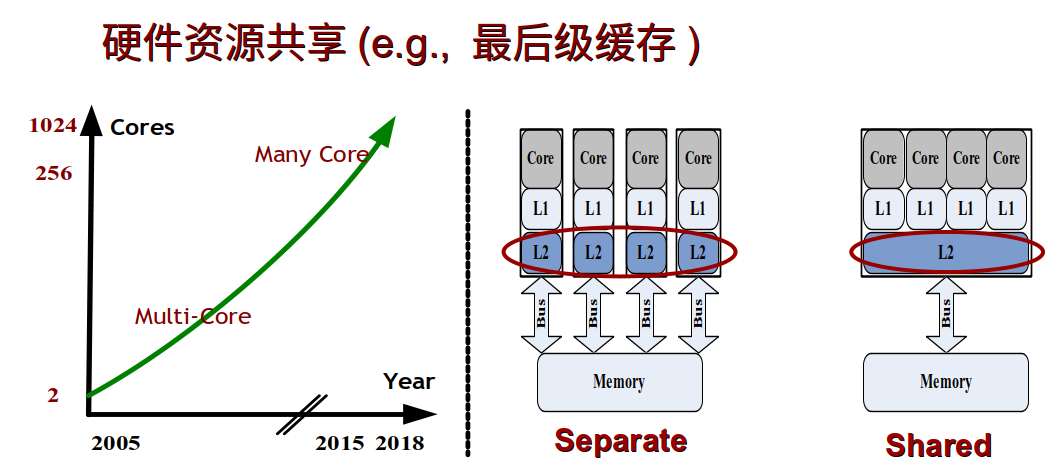
\includegraphics[width=1.\textwidth]{multicore-smp}
\end{frame}


%----------------------------------------------
\begin{frame}[plain]	
	\frametitle{Introduction}
	\Large
		NUMA 架构
%		\centering 
	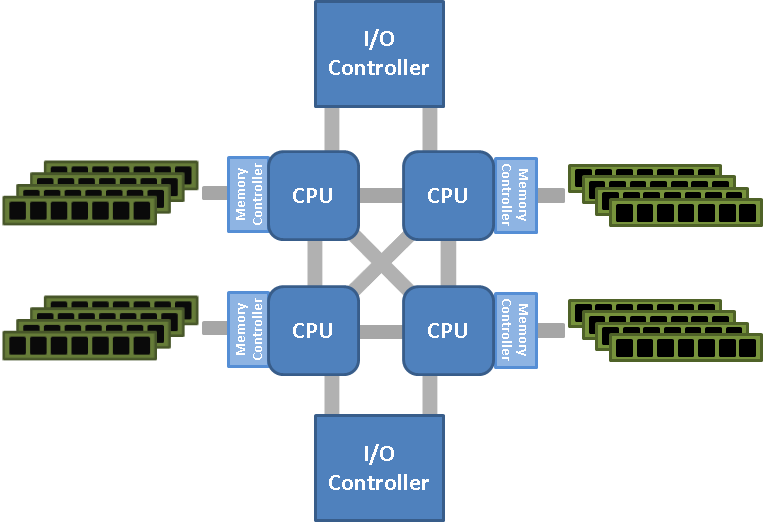
\includegraphics[width=.6\textwidth]{numa-arch}


\end{frame}

%----------------------------------------------
\begin{frame}[plain]	
	\frametitle{Introduction}

	
		\begin{columns}
		
		\begin{column}{.4\textwidth}
			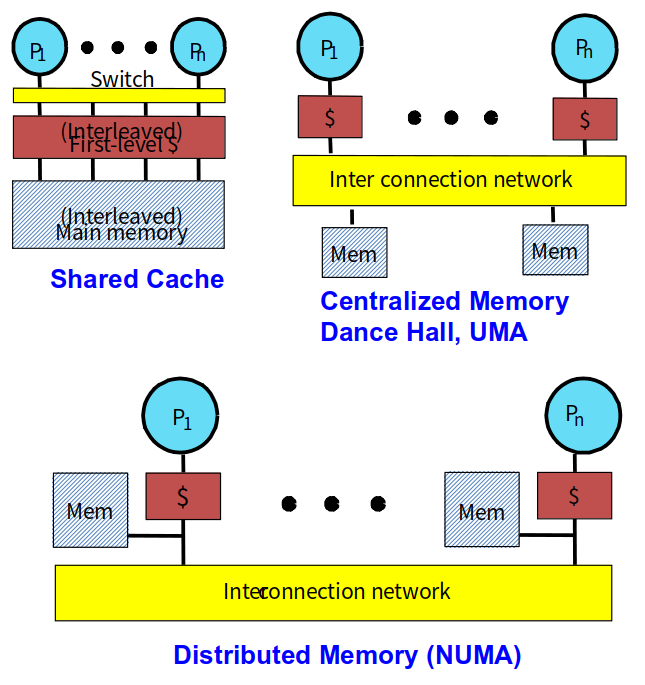
\includegraphics[width=1.\textwidth]{sharemem-archs}
		\end{column}
		\begin{column}{.6\textwidth}
				\Large \centering
			一些重要的体系结构参数数据(cycles)
			%		\centering 
			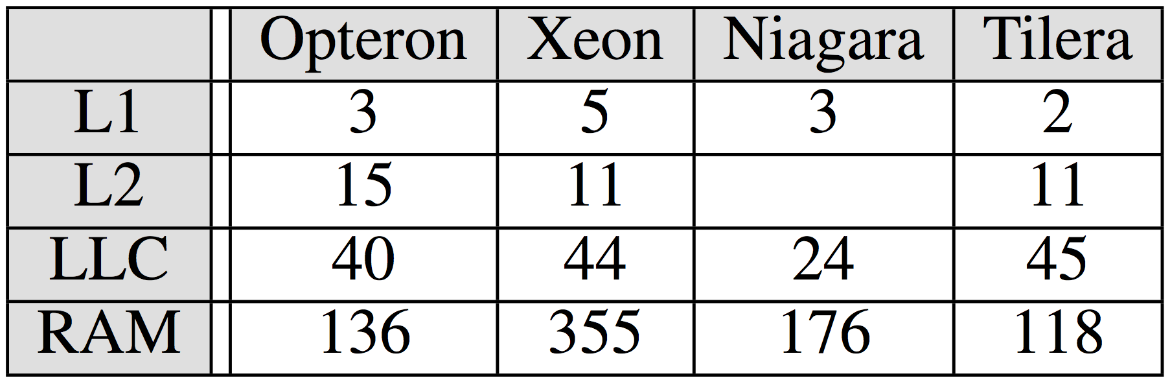
\includegraphics[width=.8\textwidth]{arch-numbers}
			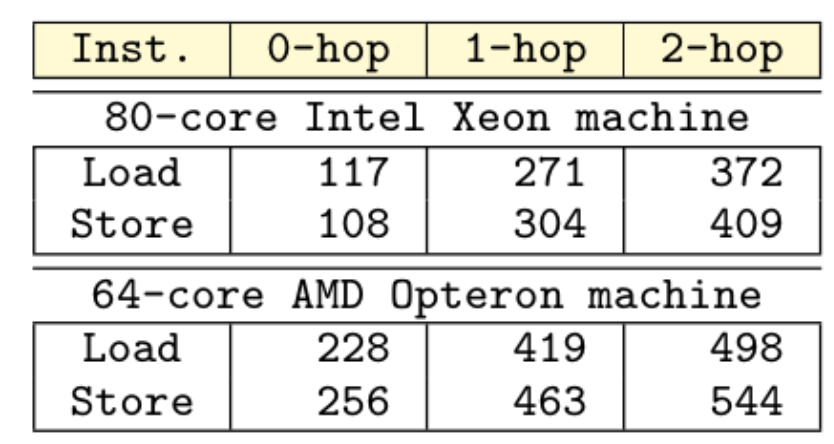
\includegraphics[width=.8\textwidth]{numa-arch-numbers}
		\end{column}
	\end{columns}
	
\end{frame}



%-------------------------------------------------


%----------------------------------------------
\begin{frame}[plain]	
	\frametitle{Introduction}
	需要分析的问题
\begin{itemize}
	\item 操作系统在多核+NUMA平台上的可扩展性能如何?
\end{itemize}	
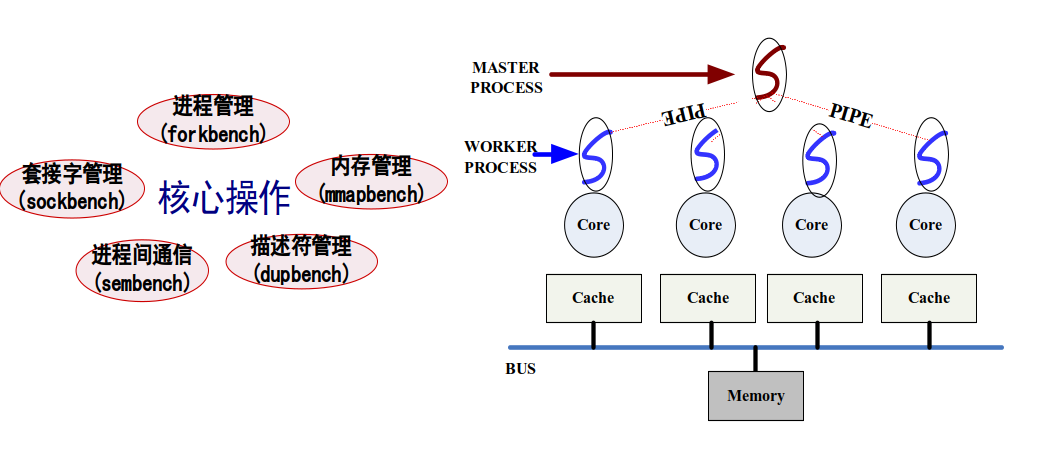
\includegraphics[width=1.\textwidth]{ostestsuits}
	
\end{frame}

%----------------------------------------------
\begin{frame}[plain]	
	\frametitle{Introduction}
	需要分析的问题
	\begin{itemize}
		\item 操作系统在多核+NUMA平台上的可扩展性能如何?
	\end{itemize}	
	mmapbench
	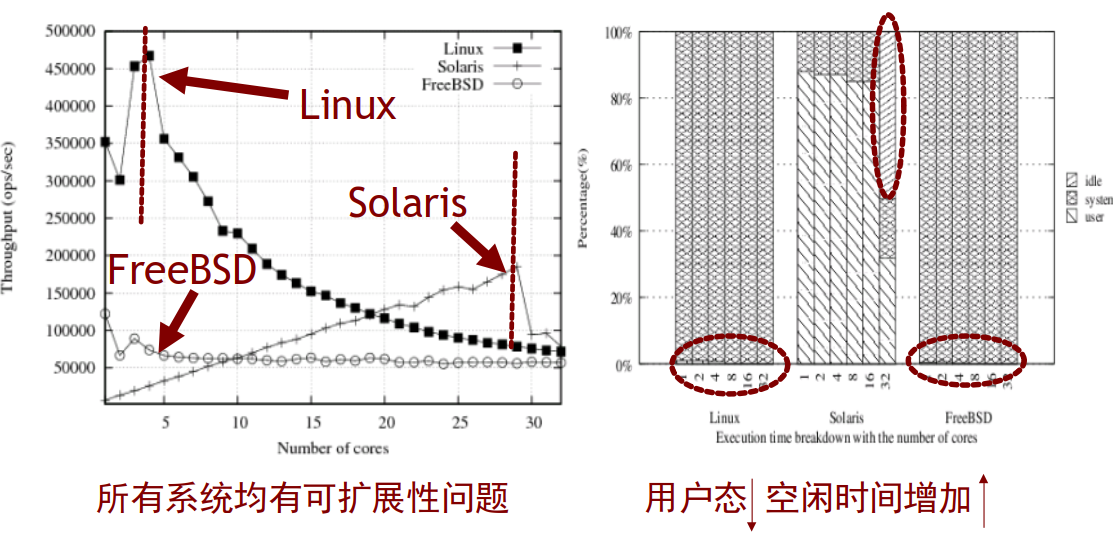
\includegraphics[width=1.\textwidth]{ostestsuits-results}
	
\end{frame}


%----------------------------------------------
\begin{frame}[plain]	
	\frametitle{Introduction}
%	需要分析的问题
%	\begin{itemize}
%		\item 操作系统在多核+NUMA平台上的可扩展性能如何?
%	\end{itemize}	

	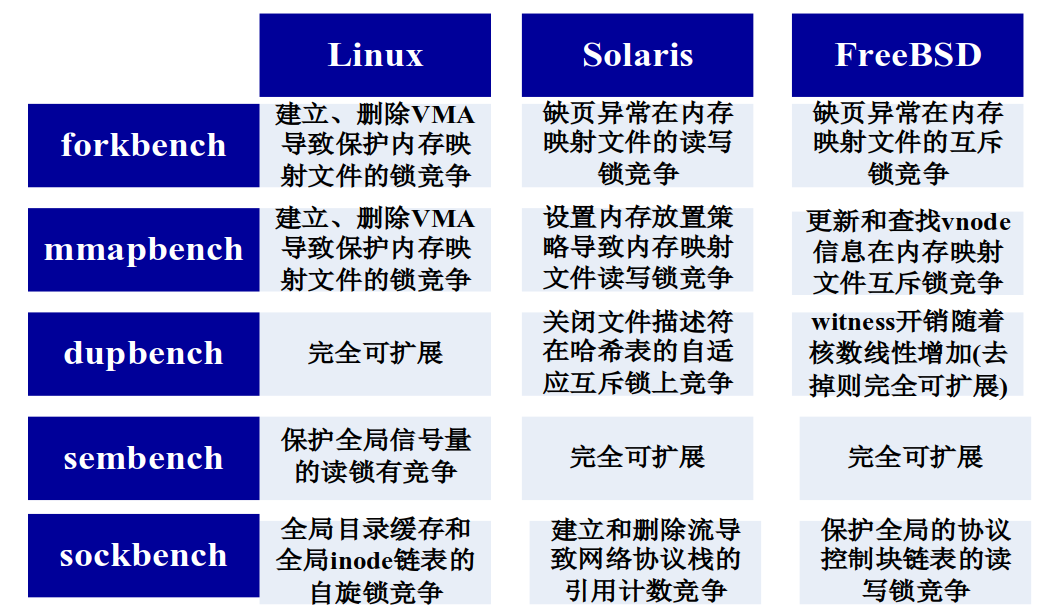
\includegraphics[width=.7\textwidth]{os-scalable-analyze}
	\begin{itemize}
		\item 操作系统中保护共享数据结构的同步原语是影响可扩展性的重要因素 
		\item 锁竞争可能导致可扩展性随着核数的增加而下降(锁颠簸现象)
	\end{itemize}
\end{frame}

%----------------------------------------------
\begin{frame}[plain]	
	\frametitle{Introduction}
	\Large \centering
	What is scalability? 
	\begin{itemize}
		\item Amdahl's law
	\end{itemize}
	
	\begin{columns}
		
		\begin{column}{.5\textwidth}
			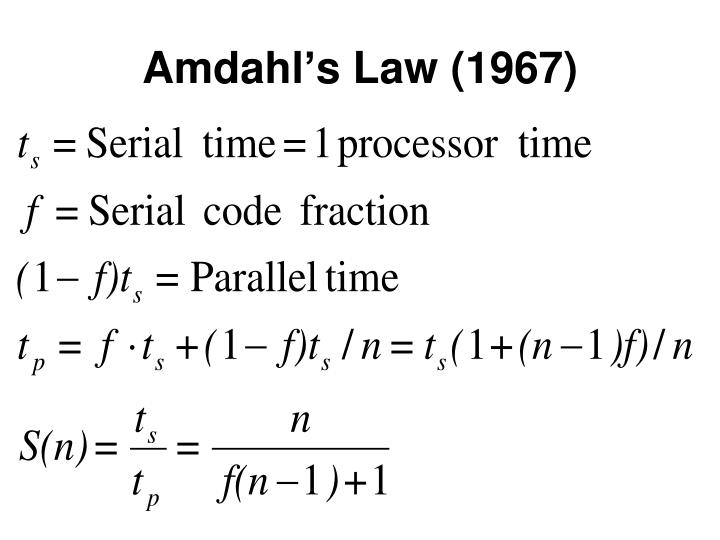
\includegraphics[width=1.\textwidth]{amdahl-s-law}
		\end{column}
		\begin{column}{.5\textwidth}
			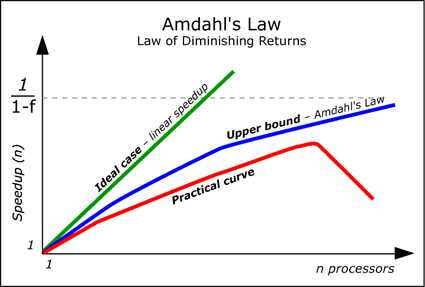
\includegraphics[width=1.\textwidth]{amdahl-s-law-graph}
		\end{column}
	\end{columns}
\end{frame}



%----------------------------------------------
\begin{frame}[plain]	
	\frametitle{Introduction}
	\Large \centering
	Locking/Mutex/Synchronization 

	
	\begin{columns}
		
		\begin{column}{.5\textwidth}
				\begin{itemize}
				\item Acquire lock
				\item critical section
				\item Release lock
			\end{itemize}
			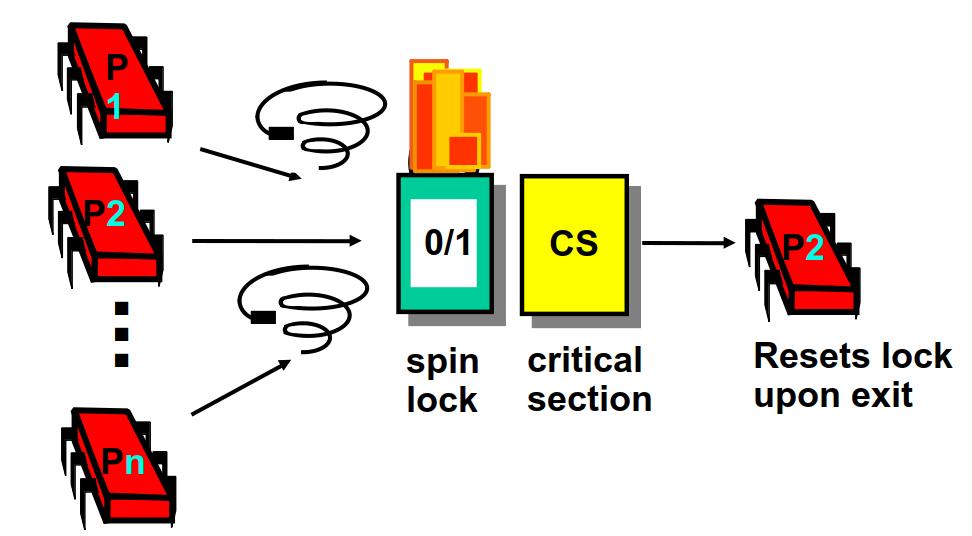
\includegraphics[width=1.\textwidth]{lock-graph}
		\end{column}
		\begin{column}{.5\textwidth}
			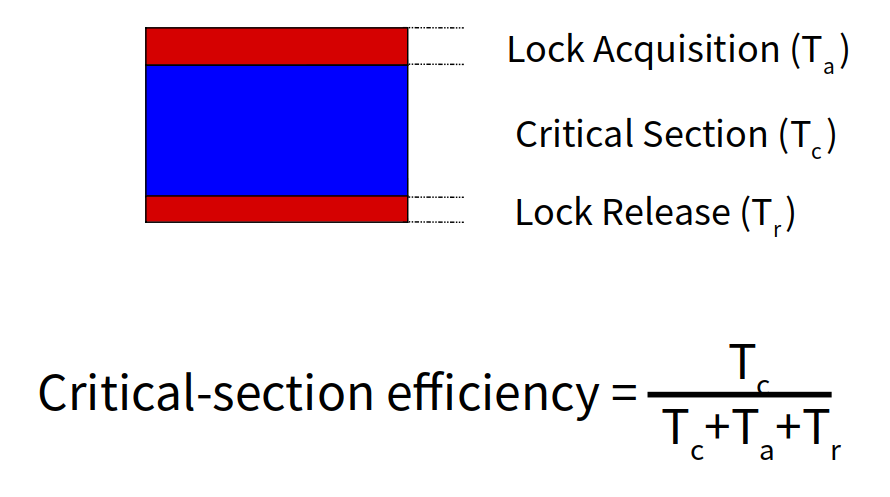
\includegraphics[width=1.\textwidth]{cirtical-section-efficiency}
		\end{column}
	\end{columns}
\end{frame}


%----------------------------------------------
\begin{frame}[plain]	
	\frametitle{Introduction}
	\centering \Large
	Various types of synchronization techniques used by the Linux
	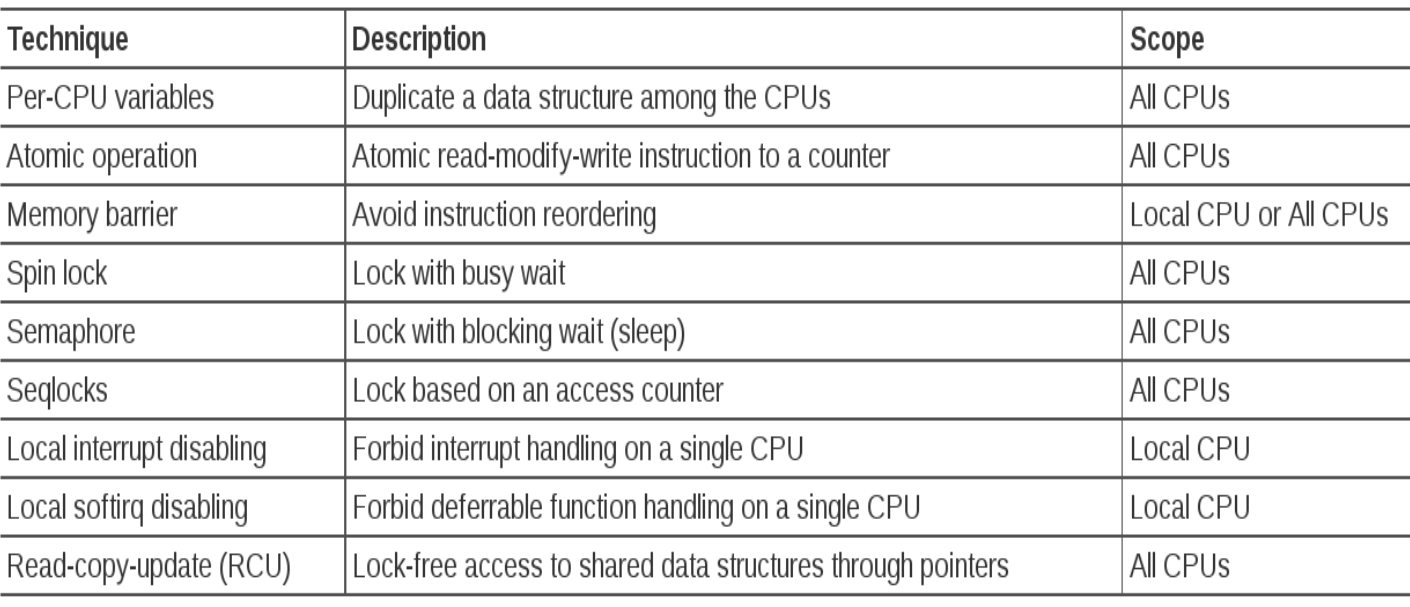
\includegraphics[width=.8\textwidth]{linux-sync-funs}

\end{frame}

%但是关于并发编程的问题你应该有所了解了,比如原子性问题,可见性问题和有序性问题。
%
%其实,原子性问题,可见性问题和有序性问题是人们抽象定义出来的。而这个抽象的底层问题就是前面提到的缓存一致性问题、处理器优化问题和指令重排问题等。
%
%这里简单回顾下这三个问题,我们说,并发编程,为了保证数据的安全,需要满足以下三个特性:
%
%原子性,是指在一个操作中,CPU 不可以在中途暂停然后再调度,即不被中断操作,要不执行完成,要不就不执行。
%可见性,是指当多个线程访问同一个变量时,一个线程修改了这个变量的值,其他线程能够立即看得到修改的值。
%有序性,即程序执行的顺序按照代码的先后顺序执行。

%-------------------------------------------------
\end{document}